% Geometry, font
\documentclass[12pt, letter]{article}
\usepackage[margin=0.8in]{geometry}
\usepackage[T1]{fontenc}
\usepackage{fourier}
\usepackage{titling}
\setlength{\droptitle}{-5em} 
\usepackage[parfill]{parskip}
\usepackage{graphicx}
\graphicspath{{figs/}}
\usepackage{hyperref}

% Math stuff
\usepackage{amssymb}
\usepackage{amsmath}
\usepackage{bm}

% Code Highlighting
\usepackage{minted}
\usemintedstyle{solarizedlight}

\author{Zach Neveu}
\title{ Problem Set 1 }

\begin{document}
\maketitle

\section{Question 1}%
\label{sec:questions}
\texttt{A}  is the correct choice. To perform leave-one-out validation, it is necessary to train the model on all data except one point, then repeat this process for every point. This requires training the model as many times as there are data points which is quite expensive computationally.

\section{Question 2}%
\label{sec:question_2}
\begin{itemize}
	\item 5 fold cross-validation * 4 regularization strengths 
	\item Hold-out method to estimate generalization error with only 1 strength
	\item Time taken: $5*4(D_{train}+D_{test})+D_{train}+D_{test}$
	\item Time taken: $21*N_{train}^2+\frac{21}{2}N_{test}^2$
	\item Time taken ($N=5000$ ): $21*(.9*5000)^2+\frac{21}{2}(.1*5000)^2$
	\item Time = $4.3575e8 = 435,750,000$
\end{itemize}

\section{Question 3}%
\label{sec:question_3}
\begin{itemize}
	\item Q1 -> Q8,Q5,Q3 -> blue,blue,red -> blue -> wrong
	\item Q2 -> Q5,Q6,Q4 -> blue,blue,red -> blue -> wrong
	\item Q3 -> Q6,Q5,Q8 -> blue,blue,blue -> blue -> wrong
	\item Q4 -> Q7,Q2,Q6 -> blue,red,blue -> blue -> wrong
	\item Q5 -> Q3,Q6,Q8 -> red,blue,blue -> blue -> right
	\item Q6 -> Q3,Q5,Q7 -> red,blue,blue -> blue -> right
	\item Q7 -> Q6,Q3,Q4 -> blue,red,red -> red -> wrong
	\item Q8 -> Q1,Q5,Q3 -> red,blue,red -> red -> wrong
	\item 2/8 total correct
\end{itemize}

\section{Question 4}%
\label{sec:question_4}
\begin{itemize}
	\item $Z = x+y$
	\item $E[Z] = E[x+y] = E[x]+E[y]$
\end{itemize}

\section{Question 5}%
\label{sec:question_5}
\begin{itemize}
	\item nslots = 38
	\item nred = 18
	\item nblack = 18
	\item p(red) = p(black) = p(win) = 18/38
	\item E(win) = p(win)*2 = 36/38*\$1 $\approx$ \$0.95
\end{itemize}

\section{Question 6}%
\label{sec:question_6}
\begin{itemize}
	\item p(cancer) = 0.007
	\item p(positive | cancer) = 0.9
	\item p(positive| no cancer) = 0.08
	\item p(cancer | positive) = p(positive | cancer) * p(cancer) / p(positive)
	\item p(cancer | positive) =  0.9*0.007 / (p(positive | cancer)*p(cancer) + p(positive | no cancer)*p(no cancer))
	\item p(cancer | positive) = 0.9*0.007 / (0.9*0.007 + 0.08*(1-0.007))
	\item p(cancer | positive) = .0734
	\item So there is a 7.34\% chance she has cancer if the mammogram comes back positive.
\end{itemize}

\section{Question 7}%
\label{sec:question_7}
\begin{itemize}
	\item $Var(y) = E[y^2]-E[y]^2$
	\item Since $1^2=1$, $Var(y) = E[y]-E[y]^2$
	\item $Var(y) = p-p^2 = p(1-p)$
\end{itemize}

\section{Question 8}%
\label{sec:question_8}
\[
	conv(x(n), y(n)) = \begin{cases}
	\frac{1}{6}(x+2)^2 & -2 \le x < 2 \\
	\frac{4}{3}x      & 2 \le x < 4 \\
	6 - \frac{1}{6}(x-2)^2 & 4 \le x < 8 \\
	0	& o.w.
	\end{cases}
\]

\begin{figure}[h]
	\centering
	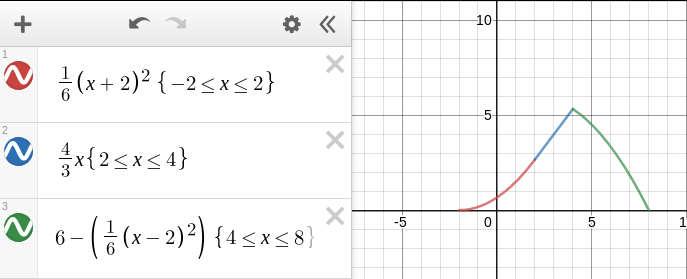
\includegraphics[width=0.8\textwidth]{conv}
	\caption{conv}
	\label{fig:conv}
\end{figure}



\section{Question 9}%
\label{sec:question_9}
\subsection*{Part A}
\[
x(t) = A\cos(2\pi F_0t+\theta) = Re(Ae^{j 2\pi F_0t+\theta}) = \frac{A}{2}\big(e^{-(j 2\pi F_0t+\theta)}+e^{j 2\pi F_0+\theta}\big)
\]
\subsection*{Part B}
Fourier Coefficients: $a_0 = 0, a_1 =  \frac{A}{2}, a_n = 0 \ for \  n > 1$

\subsection*{Part C}
Power (RMS): $\sqrt{\frac{1}{2}}A $ \\
Energy: $\infty$ since signal is not time limited and has constant amplitude

\end{document}
